\chapter{Literature Review\label{cha:chapter2}}
This chapter presents a comprehensive review of important literature relevant to the key topics of this thesis: Initially, we examine the evolution of access control. This is followed by an in-depth exploration of distributed event stores, elucidating their development, their strengths and weaknesses, and their prominence in modern distributed database systems. Subsequently, the following section explores data anonymization, highlighting general techniques as well as those specifically tailored for streaming data.


\section{Access Control\label{sec:rbac}}
Access control is a fundamental concept in information security, defining the actions that a subject, typically a user or an automated process run by a user, is authorized to perform on an object, which could be data, files, or other system resources \cite{Sandhu1994}. These actions include a variety of operations, traditionally including but not limited to, reading, writing, and executing files or data. As a critical component of system security, the methodologies and principles have been subject to extensive research and evolution over several decades. Ever adapting to the change of requirements and emerging security concerns.\par

Sahndu and Samarati's seminal work \cite{Sandhu1994} lays the foundational framework for understanding access control in the broader context of information security. They emphasize access control as an integral component of overall security, closely linked with authentification and auditing. They go on to describe the basic principles of access control, distinguishing between policies and mechanisms, focusing on the former. First, they explain the Access Control Matrix and their derivatives \acp{ACL} and Capabilities lists and ultimately Authorization Relations. The Access Control Matrix is a basic security model where rows represent subjects and columns represent objects. Each cell in this matrix specifies the actions a subject can perform on an object. However, this matrix often contains many empty cells as not all subjects interact with all objects. \acp{ACL} offer a streamlined approach by listing objects and specifying which users have what permissions. Conversely, Capabilities Lists provide a subject-focused perspective, listing subjects and their permissions for different objects. Furthermore, they analyze the prevailing standards of their time: \ac{DAC} and \ac{MAC}. In \ac{DAC} permissions are assigned by the resource owner typically in the form of \acp{ACL}. A resource owner is also at liberty to delegate the task of granting permissions to another subject. Thus, this approach does not facilitate control over the dissemination of information, however, the decentralized approach provides flexibility. \ac{MAC} on the other hand relies on a central authority to decide on all matters related to permissions. With roots in the US military, it drew inspiration from the need-to-know principle. In \ac{MAC} the flow of information is strictly regulated. Overall, the authors criticize both approaches to access control regarding their adaptability and scope. The mandatory approach was considered too rigid, the discretionary model was largely confined to research applications due to its cooperative yet autonomous focus.\par 
They appreciate the newcomer \ac{RBAC} in the space, for its discretionary flexibility and its mandatory strictness, providing a wide range of applicability, especially in commercial enterprises. A key benefit of \ac{RBAC} lies in its facilitation of smooth transitions of permissions and privileges when a user's role within an organization changes. Moreover, \ac{RBAC} simplifies the implementation of separation of duties, through mutually exclusive roles. Sahndu elaborates on \ac{RBAC} further together with Coyne \cite{Sandhu_Coyne_1994} explaining that finding a consensus in the form of a \ac{RBAC} standard requires a multidimensional view, stating that considerations regarding the nature of privileges and permissions, hierarchical roles, user assignments, privilege and permission assignment, role usage, role evolution as well as object attributes have to be made. \par
A comprehensive understanding of \ac{RBAC} requires the distinction between user groups and roles. Permissions based on user groups are a long-established practice - but do not offer the same range of functionality as role-based permissions. Ferraiolo and Kuhn \cite{ferraiolo1992role} identify two distinct differences, the first being that groups function as a discretionary mechanism, unlike roles. Access rights are assigned at the liberty of the object owner, with groups comprising users to whom the owner grants access. In contrast, roles represent a more abstract categorization of the user, allowing a single user to be associated with multiple roles. Unlike group-based access, permissions in a role-based model are assigned based on the roles themselves, not at the discretion of the resource owner. The second key difference lies in the operations associated with the permission. Groups are assigned classical file permissions as is common for an operating system e.g. read, write, execute, and own. Roles, on the other hand, refine this approach by defining 'transactions' - the authorization to execute a specific function on a set of data items. This allows for a much more nuanced and finetuned approach to access control, aligning more closely with practical requirements and daily operations. \par
Building on these insights, Sandhu further solidifies the concept of \ac{RBAC} in his pivotal work 'Role-based access control' \cite{sandhu1998role} laying the cornerstone for the formulation of a standard. In 2001, Ferraiolo et al. \cite{Ferraiolo2001} proposed a NIST standard for role-based access control, with Sandhu notably listed as a contributing author. Their goal was to bring clarity and establish well-founded, common terminology in the field of role-based access control. Their standard introduces four levels of \ac{RBAC}, each building upon the other. The foundational level, termed, 'Core \ac{RBAC}', includes basic data elements, namely users, roles, objects, operations, and permissions. Users are assigned to roles. Roles in turn are assigned permissions. Permissions are permissible operations to objects. In any given session, a user operates under a specific subset of their assigned roles. This core concept is then expanded to include hierarchies of roles, static separations of duties, and, ultimately, dynamic separations of duties. \par
Access control methodologies continue to evolve, with fine-grained access control emerging as a particularly popular approach due to its enhanced granularity in permission settings. Wang et al. \cite{wang2007correctness} examined the correctness of fine-grained access control, formulating the requirements of them being sound and secure to achieve maximum information. Other concepts include purpose-based access control for privacy protection \cite{Byun2008}. \par
An especially interesting inquiry relevant to this thesis is raised by Chaudhuri et al. in \cite{chaudhuri2011database}. They ask whether there is common ground between database access control and privacy. Despite their apparent relation, these two are seldom addressed together. In their journal article, they expand on the differential privacy notion with noisy views. Differential privacy requires that computations are formally equivalent when performed with or without any single record. Noisy views refer to the technique of adding noise to aggregate data in a database, thereby enhancing privacy. This innovative combination implemented on a database server level seems promising in bridging the gap between access control and privacy. This approach of harmonizing access control and privacy aligns closely with the objectives pursued in this thesis.



\section{Distributed Event Stores}
In modern times data is being produced at an unprecedented rate and volume. A significant portion of that data is so-called 'streaming data'. Streaming data is continuously generated, often in high volumes and at high velocity, from various sources. Its distinguishing characteristic, however, lies in its continuous flow and boundless nature. It additionally requires real-time or near-real-time processing as relevancy is key. Sources of streaming data include \ac{IoT} devices, log files, financial transactions, and social media platforms. One of the key challenges of streaming data is the need for systems that can process and analyze the data as soon as it arrives. This difficulty is exacerbated by the volume, velocity, and variety (the three Vs of Big Data) of the data. Moreover, streaming data often requires a different approach to data management and storage. Since the data is continually flowing, it is infeasible to store all incoming data indefinitely. \par
Traditionally, relational databases have been the go-to with Oracle \cite{oracle} and MySQL \cite{mysql} as the dominating database management systems \cite{dbms_statistics}. Over time, relational databases have evolved. Initially, their primary focus was enabling high-speed transaction processing, as illustrated by Selinger et al. in 1979 \cite{selinger1979access}. The emergence of unstructured data, as is common in streaming data, for instance, has led to a shift away from relational databases to column-based or more generally NoSQL databases. Prominent examples of such databases include Apache Cassandra \cite{cassandra}, Cloud Bigtable \cite{cloud_bigtable}, Amazon Redshift \cite{amazon_redshift}, and MongoDB \cite{mongo_db}. The immediate processing and decision-making requirements of streaming data can oftentimes not be met by these types of databases. Specifically, managing time-ordered events and executing temporal queries present significant challenges. Additionally, streaming data necessitates robust transactional guarantees in addition to complex event processing capabilities. This poses another challenge to NoSQL databases. Ultimately, the high throughput and low latency demands on top of the aforementioned requirements are enough to require a new model entirely. \par
The architectural pattern of event sourcing emerges. It involves storing the state changes of an application as a sequence of events. Instead of keeping the current state of data in a database, every change (or event) that affects the system's state is captured and stored. These events are immutable, meaning once they are stored they cannot be changed. A principal advantage of event sourcing thus lies in the reproducibility of system changes. Events can be replayed to reconstruct the system state at any point in time. This is particularly useful for debugging, auditing, and understanding the sequence of actions that led to a particular state. \par
Numerous entities have integrated event sourcing into their database designs. Notably, Greg Young, a pioneer of event sourcing, developed EventStoreDB \cite{eventstore_db}. Nowadays, there are commercial as well as open-source solutions available, offering comprehensive capabilities for event storage. To facilitate scalability and fault-tolerance most opt for a distributed approach. Prominent \acp{DES} include Apache Kafka \cite{kafka}, Amazon Kinesis \cite{amazon_kinesis}, RabbitMQ \cite{rabbit_mq} and Apache Pulsar \cite{pulsar}. We have selected Apache Kafka as the leading example of our research. Its scalability and reliability, while maintaining low latency and high throughput have established Kafka as the de facto standard in message broking. Combined with its compatibility with essentially all stream processing frameworks, albeit offering its stream processing framework Kafka Streams, Kafka is one of the leaders in big data processing technologies worldwide. Its utilization spans multiple sectors, including Fortune 100 companies, governments, and healthcare. Furthermore, as an open-source technology, Apache Kafka offers
a rich set of tools and an active community. This allows a more thorough exploration of practical implementations simultaneously staying grounded in real-world applicability.

\subsection{Apache Kafka}
Let us begin by taking a look at Kafka's architecture shown in Figure \ref{fig:kafka}. There is quite a bit of Kafka terminology involved, in the following written in cursive. 

\begin{figure}[ht]
   \begin{adjustbox}{center}
   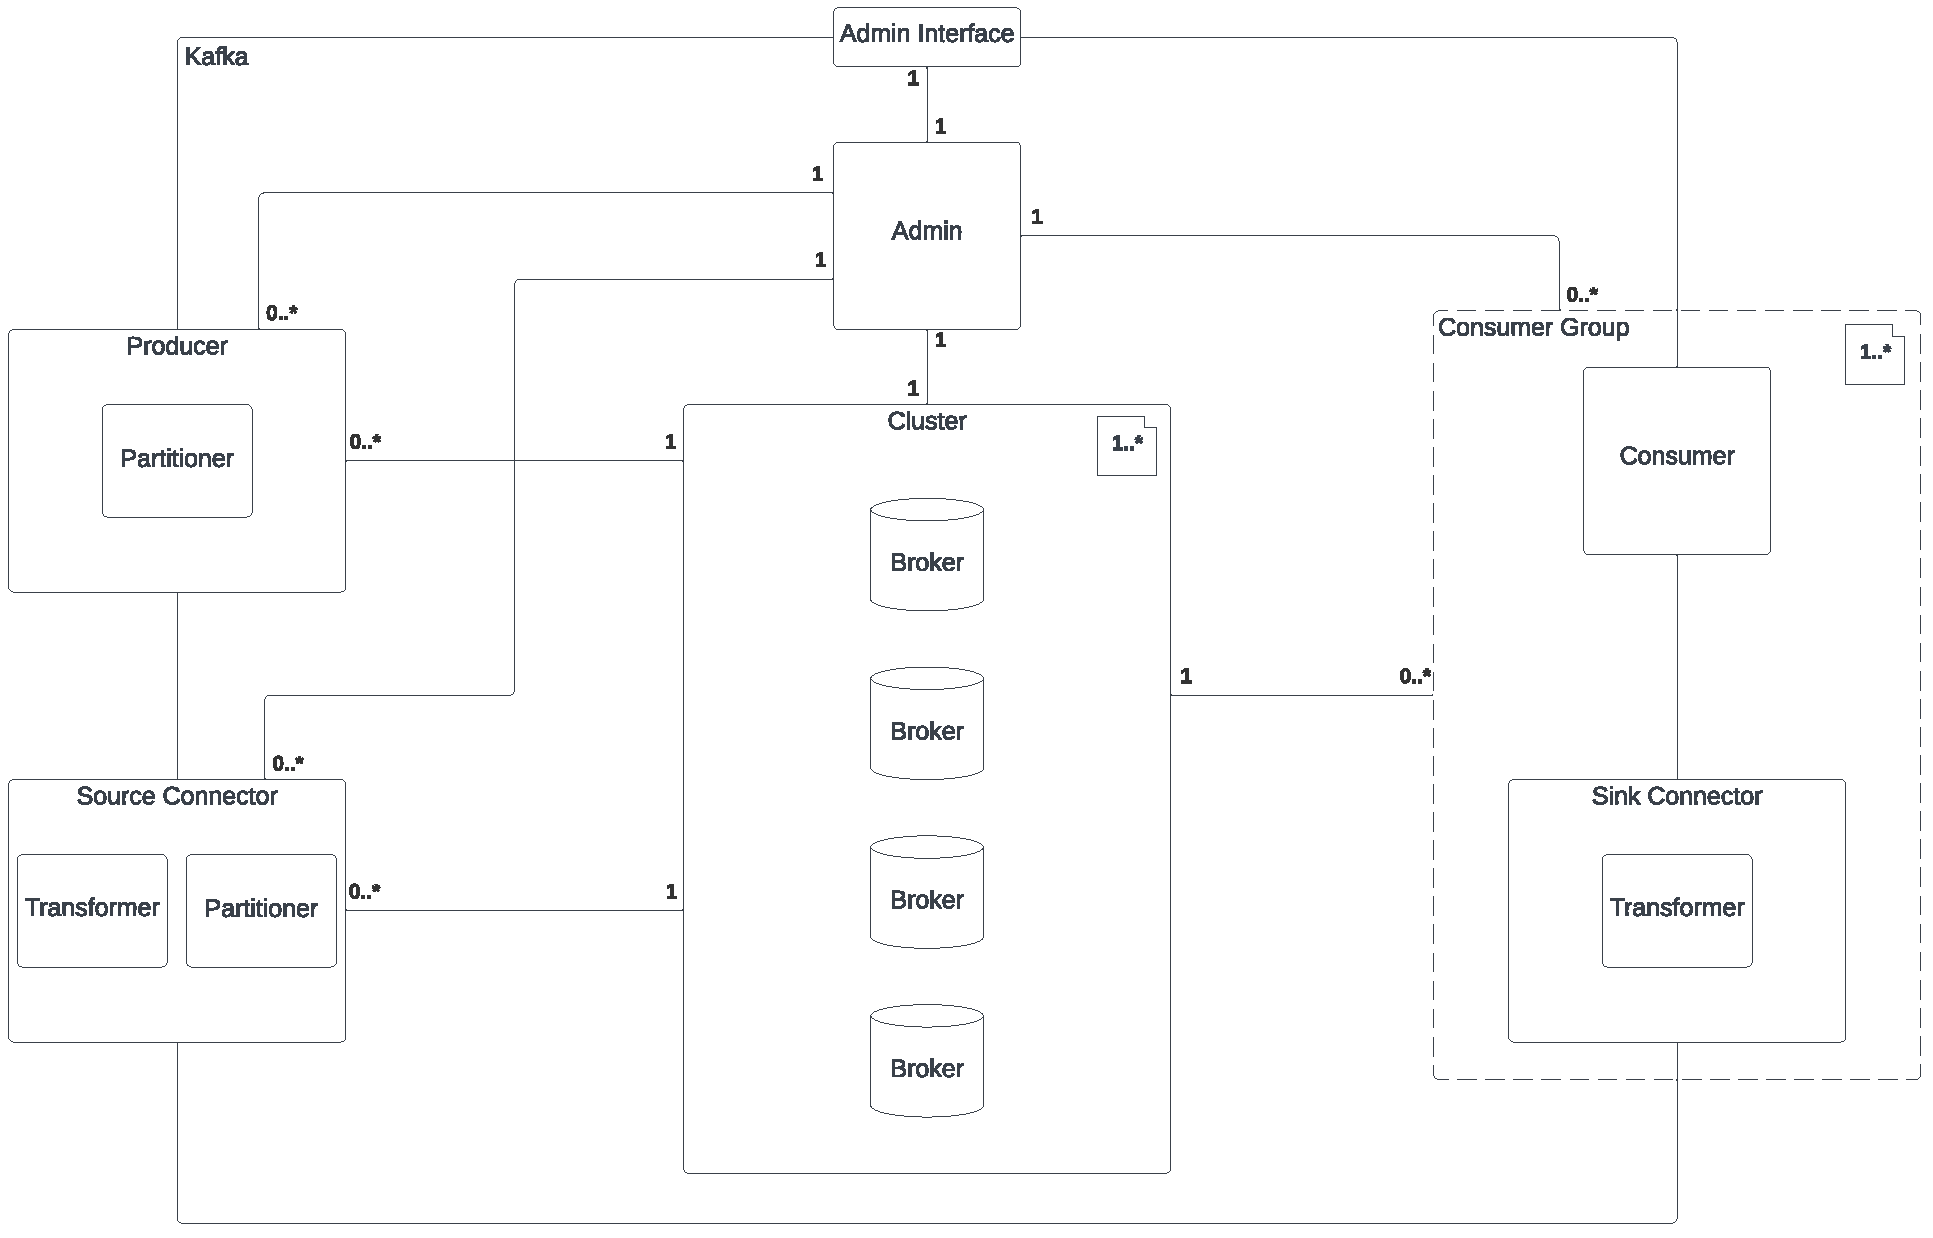
\includegraphics[width=0.8\pdfpagewidth]{img/Kafka_Diagram.pdf}
   \end{adjustbox}
   \caption{Apache Kafka Architecture and Terminology. The links between components have been enhanced with cardinalities to provide more context. \label{fig:kafka}}
\end{figure}

At the core is the \textit{Cluster}, containing at least one \textit{Broker} (database), this is denoted with the note in the top right corner reading '1..*'. As a cluster, they function as distributed storage. However, they deal exclusively with streaming data. A singular stream of related events is termed \textit{Topic}, produced and distributed across the individual Brokers according to strategies delineated by the administration component. For topic production, a \textit{Producer} must be developed by the user to format the raw data. Alternatively, users can employ \textit{Connectors} that interface external systems with Kafka, thus relieving users of data transformation tasks. These connectors are available in a plug-and-play fashion, and the \textit{Kafka Connect} framework allows for the creation of custom connectors. \textit{Consumers} retrieve topics, operating collectively within \textit{Consumer Groups}. Kafka provides three distinct delivery semantics — 'at least once', 'at most once', and 'exactly once' — which refer to how often a singular event is delivered to each consumer group. On the consumer side, similarly to Producers, a \textit{Kafka Consumer} requires user development, although connectors for integrating Kafka with external systems are available. Note that custom Consumers and Connectors can coexist in on Consumer Group. The administration is available through a \textit{Kafka Admin} framework. However, simply using the Kafka Admin framework requires significant development overhead. Instead, other frameworks are brought in to adopt this task. \par 

There are several tasks that the administration unit of Kafka has to accomplish. These administrative tasks must be made configurable for the system administrator within the Kafka environment. The responsibilities include the following: 

\begin{enumerate}
   \item \textbf{Cluster configuration}\\It must be in close communication with the brokers. It must be possible to add and delete individual brokers to the cluster.
   \item \textbf{Topic Control}\\Topics must be creatable and deletable. Topics are associated with producers and consumer groups. In particular, the offsets for consumer groups must be monitored. Typically, this is done in an additional "consumer offsets" topic. Here consumer groups are mapped to their offset. Consumer groups periodically publish on this specific topic whenever they consume messages from their respective topics.  
   \item \textbf{Partition Strategy}\\The partition strategy for producers must be communicated. Partitions need to be assigned to brokers. 
   \item \textbf{Replication Strategy}\\To ensure reliability partitions need to be replicated. There is a partition leader stored on one broker and replications on several other brokers. The administration must be able to select the replication strategy.
   \item \textbf{Access Control}\\Access control must be enforceable for producers, consumers, and particularly for administrative operations.  
   \item \textbf{Fault-tolerant}\\The administration component itself must be robust and reliable.
\end{enumerate}

While technically all these requirements can be met simply using the Kafka Admin framework, Kafka themselves do not recommend it. Up until Kafka Version 3.3 (released in August 2022), Kafka advised the delegation of the administration to another framework called \textit{Apache ZooKeeper}. ZooKeeper is an open-source centralized service for synchronizing distributed systems, maintaining configuration information, and providing group services. It facilitates the communication of the various components with each other through hierarchical namespaces. Each namespace corresponds to a node within a hierarchical tree structure. A node on its own can simultaneously have children and data. As ZooKeeper is designed for configuration information the data associated with a node is expected to be small (Byte to Kilobyte in size). For instance, ZooKeeper creates nodes for each broker and stores its configuration as data. In a separate node, it stores information about each topic including its partitions, the assignments of partitions to brokers, and the replication logic. These correlations enable ZooKeeper to maintain system operations and adapt to changes. Each node also encompasses a \ac{ACL} that governs the access to the node's data and its children. The change of the ACL of a topic node for instance would affect the access control for the consumption of that topic. ZooKeeper relies on replication to ensure fault tolerance. In addition, watches are created to detect failures in individual nodes. With all this in place, ZooKeeper makes the following guarantees: Sequential Consistency, Atomicity, Single System Image, Reliability and Timeliness. Altogether, it provides all responsibilities as described in the prior.\par
Apache Kafka, however, has created its own administration component called \textit{KRaft}. Instead of administering the cluster externally, it delegates this responsibility to the brokers. They store the necessary metadata for maintenance and administration alongside the topic partitions. Again replication and partition are utilized to ensure durability. This approach significantly reduces overhead, as it obviates the need to maintain and store separate ZooKeeper nodes. KRaft has been introduced in Kafka Version 3.3 and is production ready as of Version 3.5 (released June 2023). However, it may be reasonably anticipated that the adoption of this new administrative approach within production servers will occur over several years.



\section{Anonymization for Streaming Data\label{sec:anon}\label{lit:data_streaming}}
Protecting privacy is an increasing concern for companies that rely on processing data. With extensive legislation in place across the globe, data scientists and data engineers alike are tasked with securing their users' data. The key requirement for privacy is restricting the reidentification of an individual with a record. Typically, the attributes in a single record can be categorized into direct identifiers also called \ac{PII}, indirect identifiers called quasi-identifiers, and the remaining, sensitive data \cite{gdpr_recital_26}. Anonymization takes on different forms in achieving the task of preventing reidentification. \par 

One approach to anonymization is to use cryptographic methods to make it unreadable for individuals without access to the key. Depending on the concrete cryptographic function, this can be an expensive yet secure way of doing it. Streaming data, however, is transient and needs to be processed in real-time. Typically, this involves augmenting, testing, or otherwise transforming the data. This process is made more difficult if not impossible with encrypted data as in its encrypted form it contains essentially no information except that it is there. Decrypting the data again before processing and encrypting it again after is cumbersome and results in the processing of unanonymized data, which defeats the purpose of anonymizing data with cryptographic methods in the first place. \par
 
An alternative approach involves employing masking functions, which alter the original data values, thereby obfuscating them and making it more challenging for unauthorized entities to discern the true information. In contrast to cryptographic functions, this is generally a cheaper approach, but the resulting protection is highly dependent on the masking function and its application. In general, simple masking functions are well-suited for data stream handling, as they modify single data points and integrate seamlessly into the data pipeline. Complex masking functions, such as those performing aggregations based on multiple data points simultaneously, require a distinct approach. An unbounded data stream must be discretized into finite sets of data for these functions to operate effectively. Modern data stream handlers, such as \ac{DES}, typically employ 'windowing' techniques. Windowing segments an unbounded stream into discrete windows of record collections. These may vary in size, overlap, and basis (periods, sessions, or states). The scope of this concept is extensive, encompassing a vast array of methodologies and applications. Researchers have developed specialized adaptations of established concepts to address the unique challenges of streaming data. \par
In the following, we survey the most prevalent masking functions, describing their operational principles and applications. Subsequently, we take a closer look at CASTLE \cite{Cao2008}, an algorithm specifically designed to achieve k-anonymity for anonymizing streaming data. 

\subsection{Masking Functions\label{sec:masking_functions}}
Initially, we establish a basic understanding of key terms essential for this discussion. In this context, a \textit{datum} refers to a single piece of information e.g. a singular entry of a database or any one event of a data stream. Synonymous with it also used the word \textit{tuple}. A tuple is composed of one or multiple \textit{attributes}. The names of the attributes are typically used as keys for identification of the attribute within the tuple. It is customary for individual tuples to be part of a bigger collection. In the static context, they are collected in databases and grouped in tables. Data streams work analogous to dynamic operations. All tuples of the same database table or data stream are required to follow the same pattern. This refers to the sequence of attributes of each tuple. This pattern is fixed in a data schema associated with the table or stream. Sometimes it is appended to each datum in the form of a header. As this substantially increases the size of each datum it is more common to define it once in the initialization step of the database table or data stream. \par
Having established the terminology let us begin by introducing prevalent masking functions:\par

\textbf{Suppression} aims to effectively delete the value of a tuple's attribute by replacing it with a meaningless character, most commonly the asterisk \textit{*}. It is important to note, that actually removing the attribute from the tuple or replacing it with a null value would violate the data schema and thus negatively impact operability. The asterisk does the trick while maintaining the data schema. To work, Suppression only requires a non-empty set of keys for the attributes that are supposed to be suppressed as parameters. Naturally, it leads to total information loss of the specified fields. This can be particularly useful for fields containing \ac{PII} like a person's home address as shown in Figure \ref{fig:suppression}. 

\bigskip

\begin{figure}[ht]
    \begin{center}
    \footnotesize{
        \renewcommand{\arraystretch}{1.5}
        \begin{tabular}{|c|}
            \hline
            address \\
            \hline
            Smith Street 3 \\
            \hline
            \end{tabular}
            \quad $\longrightarrow$ \quad
            \begin{tabular}{|c|}
            \hline
            address \\
            \hline
            * \\
            \hline
        \end{tabular}
    }
    \end{center}
    \caption{Example of suppression of an attribute.\label{fig:suppression}}
\end{figure}

A similar approach is applied in \textbf{Blurring}. Here, the value of an attribute is replaced with arbitrary characters, typically \textit{X}s. It is distinguishable from Suppression in that not all characters of the value have to be replaced and even the amount of characters can remain the same. Imagine a user at the checkout of an online store that they have already purchased goods at prior to this session. Here the credit card information of that user was saved as part of the agreement from the previous session. The user is then given the option to use that credit card again, with it being specified as a sequence of blurred characters with only the last three digits in plain text as shown in Figure \ref{fig:blurring}. This allows the user to double-check the card information without exposing the credit card number to the network, screen captures, or bystanders. This operation also leads to high information loss but retains some usability of the original value. The parameters for Blurring include the keys to blur as well as optionally the number of characters and whether the amount of characters is to be maintained. Note, that setting the parameters to blur all characters and reduce the amount to one is equal in functionality to Suppression. 

\bigskip

\begin{figure}[ht]
    \begin{center}
    \footnotesize{
        \renewcommand{\arraystretch}{1.5}
        \begin{tabular}{|c|}
            \hline
            credit card \\
            \hline
            1234 5678 9123 4567 \\
            \hline
            \end{tabular}
            \quad $\longrightarrow$ \quad
            \begin{tabular}{|c|}
            \hline
            credit card \\
            \hline
            XXXX XXXX XXXX X567 \\
            \hline
        \end{tabular}
    }
    \end{center}
    \caption{Example of blurring of an attribute.\label{fig:blurring}}
\end{figure}

\textbf{Substitution} replaces the value of the specified attribute with a predefined substitute. Figure \ref{fig:substitution} shows an example where a name is switched out with an arbitrary fake name from a provided substitution list. While this masking function leads to substantial information loss, it seemingly maintains the integrity of the data from an outsider's perspective. This can make the data easier to work with, while still ensuring anonymity. As parameters, the keys for the attributes that are supposed to be substituted are required in tandem with the intended substitutes. 

\bigskip

\begin{figure}[ht]
    \begin{center}
    \footnotesize{
        \renewcommand{\arraystretch}{1.5}
        \begin{tabular}{|c|}
            \hline
            name \\
            \hline
            Martin Smith \\
            \hline
            \end{tabular}
            \quad $\longrightarrow$ \quad
            \begin{tabular}{|c|}
            \hline
            name \\
            \hline
            John Doe \\
            \hline
        \end{tabular}
    }
    \end{center}
    \caption{Example of substitution of an attribute.\label{fig:substitution}}
\end{figure}

An alternative approach is \textbf{Tokenization}. Here, values are also substituted, but not with some arbitrary replacement. Instead, the substitute is a specific token. These tokens can be reversed to restore the original value as long as a key is known with which the token was created. There are different approaches to achieve this. The first one coming to mind is a database mapping token to the hash of the original value. Only access to the database as well as the hashing function will yield the correct original value from the token. Another approach is to omit the database and instead use a more sophisticated cryptographic algorithm to create the token, effectively encrypting the data. An additional, less computationally intensive method involves the use of a hashmap, where original values are associated with randomly generated character sequences. This approach, while simpler, still provides a level of security by obfuscating the original values. Each method has its trade-offs: while the database and cryptographic approaches ensure a robust security level, they necessitate significant storage and computing resources. On the other hand, the hashmap approach, though less resource-intensive, might offer a slightly reduced security level. This makes the choice of method dependent on the sensitivity of the data and the available resources. For instance, highly sensitive information, such as passwords, might necessitate more resource-intensive methods, as depicted in Figure \ref{fig:tokenization}.

\bigskip

\begin{figure}[ht]
    \begin{center}
    \footnotesize{
        \renewcommand{\arraystretch}{1.5}
        \begin{tabular}{|c|}
            \hline
            password \\
            \hline
            MyPassword1 \\
            \hline
            \end{tabular}
            \quad $\longrightarrow$ \quad
            \begin{tabular}{|c|}
            \hline
            password \\
            \hline
            d9f4c3b72c7935e5 \\
            \hline
        \end{tabular}
    }
    \end{center}
    \caption{Example of tokenization of an attribute.\label{fig:tokenization}}
\end{figure}

One of the most common masking functions is \textbf{Generalization}. Here, the value of an attribute is abstracted to a more general value. This effectively reduces the information - but does not remove it entirely. For example, a datum with a residency field could generalize the exact location to a broader one. Instead of Berlin, it would read Germany as shown in Figure \ref{fig:generalization}. This could then be even further generalized to Europe and so forth. Typically, entire generalization hierarchies are provided as parameters to facilitate this. These hierarchies must be exhaustive of all possible arising values if no default is provided as a generalization is ambiguous. These complete generalization hierarchies are required as parameters in addition to their respective attribute key. 

\bigskip

\begin{figure}[ht]
    \begin{center}
    \footnotesize{
        \renewcommand{\arraystretch}{1.5}
        \begin{tabular}{|c|}
            \hline
            residency \\
            \hline
            Berlin \\
            \hline
            \end{tabular}
            \quad $\longrightarrow$ \quad
            \begin{tabular}{|c|}
            \hline
            residency \\
            \hline
            Germany \\
            \hline
        \end{tabular}
    }
    \end{center}
    \caption{Example of the generalization of an attribute.\label{fig:generalization}}
\end{figure}

A special case of Generalization is \textbf{Bucketizing}. It functions similarly, but exclusively for numerical values. Ranges replace specific values in the tuple. Figure \ref{fig:bucketizing} shows an example where the age 27 is bucketized to the range {[20 - 30]}. Only a moderate amount of information is lost with this masking function. To deploy, it requires the bucket sizes as well as the attribute keys. 

\bigskip

\begin{figure}[ht]
    \begin{center}
    \footnotesize{
        \renewcommand{\arraystretch}{1.5}
        \begin{tabular}{|c|}
            \hline
            age \\
            \hline
            27 \\
            \hline
            \end{tabular}
            \quad $\longrightarrow$ \quad
            \begin{tabular}{|c|}
            \hline
            age \\
            \hline
            {[20 - 30]} \\
            \hline
        \end{tabular}
    }
    \end{center}
    \caption{Example of bucketizing of an attribute.\label{fig:bucketizing}}
\end{figure}

Finally, there are the \textbf{Noise Methods}. While they can also be applied to some effect on categorical attributes, they are mostly applied to numerical data. The idea is to modify the original values by adding noise. Typically, this noise is chosen randomly from a distribution. The standard deviation will then define how much each data point can diverge from the original value. Utilizing the normal distribution with mean $0$ would ensure that the data over time would retain its mean and variance. The result will invalidate individual tuples but preserve the overall spread of the data in the long run. As an example, Figure \ref{fig:noise} shows noise added to two attributes of a tuple. Note that with no loss to the generality, one is decreased, while the other increases. 

\bigskip

\begin{figure}[ht]
    \begin{center}
    \footnotesize{
        \renewcommand{\arraystretch}{1.5}
        \begin{tabular}{|c|c|}
            \hline
            height & weight \\
            \hline
            185 & 83 \\
            \hline
            \end{tabular}
            \quad $\longrightarrow$ \quad
            \begin{tabular}{|c|c|}
            \hline
            height & weight  \\
            \hline
            181 & 84\\
            \hline
        \end{tabular}
    }
    \end{center}
    \caption{Example of adding noise.\label{fig:noise}}
\end{figure}

The aforementioned masking functions are applied to a single value within a record. There are more complex masking functions that go beyond this. For instance \textbf{Conditional Substitution} extends this by requiring a certain condition to be met for a masking to occur. Also, masking functions are considering multiple records at the same time. \textbf{Aggregation} is a familiar example where values of multiple records are aggregated with a specified method. One of the widely accepted models for preserving the privacy of data subjects in the dataset is \textbf{k-anonymity}. Introduced by Sweeney \cite{sweeney2002kanonymity}, the k-anonymity model necessitates that any record in a collection is indistinguishable from at least $k-1$ other records regarding their indirect identifiers. This model has been revised in the past, with further requirements as in the diversity of distinct sensitive values and maintaining the spread within the dataset within each subgroup of values. All these more complex masking functions rely upon and utilize the masking functions depicted in these subsections. They are the foundation of masking functions overall. The anonymization techniques we have just described provide further protection and are of great use at a cost of decreased performance.

\subsection{K-Anonymity through CASTLE\label{lit:castle}}
Created by Cao et al. \cite{Cao2008}, CASTLE is a targeted solution for k-anonymity within data streams. CASTLE stands for Continuously Anonymizing STreaming data via adaptive clustering. Streaming data differs from static databases in two key aspects: first, it is unbounded, necessitating an approach that can handle data of indeterminate size. The second distinction is that streaming data is append-only; that is, entries in a data stream are not modified or deleted once added. However, the significance of entries may diminish over time, a factor that the authors of CASTLE address by focusing on the \textit{freshness} of the data. They do this by defining a streaming variant of k-anonymity called $k_s$-anonymity.\par 
Each tuple $t$ of a stream $S$ consists, as always, of personally identying attributes $p_1, \dots, p_n$, quasi-identifiers $q_1, \dots, q_n$ and sensitive attributes $s_1,\dots, s_n$. Additionally, it is given another attribute, the position $p$ in $S$. The anonymized result of the stream $S$ is termed $S_{out}$. Given a position $P$, the authors consider $S_{out}$ \textit{$k_s$ anonymized up to P} if the collection of all tuples with $t.p \le P$ in $S_{out}$ is k-anonymized. To further facilitate the requirement of freshness they add a $\delta$-constraint to their scheme. It says that any such stream $S$ satisfied the $\delta$-constraint if all tuples with a position less than $t.p - \delta$ are already in $S_{out}$. Keep in mind that there is a time difference, the processing time, between $S$ and $S_{out}$. The algorithm consumes the plaintext stream $S$ one tuple at a time and produces the anonymized stream $S_{out}$ in batches. The $\delta$ constraint limits the number of tuples that are being processed by CASTLE at any one time and subsequently ensures that fresh data is produced to $S_{out}$. \par
Minimizing information loss is important and for k-anonymity the only leeway lies within the quasi-identifiers as they are generalized. Sensitive attributes remain untouched and \ac{PII} is suppressed. To be able to minimize information loss, it first has to be quantified. For a numerical attribute $q_i$ and the generalization $g$ to the range $[l,u]$, from the domain $[L, U]$ of $q_i$, the corresponding information loss is defined by the authors as follows: 

\begin{center}
    $VInfoLoss(g) = \frac{u - l}{U - L}$
\end{center}

The information loss for categorical attributes is calculated according to their generalization hierarchy. Figure \ref{fig:residency_hierarchy} shows the generalization hierarchy of an exemplary attribute \textit{residency} referring to the geographical location of a person's residency. 


\begin{figure}[ht]
    \begin{tikzpicture}[node distance=0.97cm]
        \tikzstyle{line} = [draw, -latex']
        \node (Berlin) {Berlin};
        \node[right=of Berlin] (Stuttgart) {Stuttgart};
        \node[below=of Berlin, yshift=0.5cm] at ($(Berlin)!0.5!(Stuttgart)$) (Munich) {Munich};
        \node[right=of Stuttgart] (Madrid) {Madrid};
        \node[right=of Madrid] (Bilbao) {Bilbao};
        \node[below =of Madrid, yshift=0.5cm] at ($(Madrid)!0.5!(Bilbao)$) (Barcelona) {Barcelona};
        \node[right=of Bilbao] (Glasgow) {Glasgow};
        \node[right=of Glasgow] (London) {London};
        \node[below =of Glasgow, yshift=0.5cm] at ($(Glasgow)!0.5!(London)$) (Manchester) {Manchester};

        \node[above=of Berlin] at ($(Berlin)!0.5!(Stuttgart)$) (Germany) {Germany};
        \node[above=of Madrid] at ($(Madrid)!0.5!(Bilbao)$) (Spain) {Spain};
        \node[above=of Glasgow] at ($(Glasgow)!0.5!(London)$) (UK) {UK};

        \node[above=of Germany] at ($(Germany)!0.5!(Spain)$) (EU) {EU};
        
        \node[above=of EU, yshift=0.25cm] at ($(EU)!0.5!(UK)$) (Europe) {Europe};

        % Paths
        \path [line] (Berlin) -- (Germany);
        \path [line] (Munich) -- (Germany);
        \path [line] (Stuttgart) -- (Germany);
        \path [line] (Madrid) -- (Spain);
        \path [line] (Barcelona) -- (Spain);
        \path [line] (Bilbao) -- (Spain);
        \path [line] (Glasgow) -- (UK);
        \path [line] (Manchester) -- (UK);
        \path [line] (London) -- (UK);

        \path [line] (Germany) -- (EU);
        \path [line] (Spain) -- (EU);

        \path[line] (EU) -- (Europe);
        \path[line] (UK) -- (Europe);


    \end{tikzpicture}
    \caption{Generalization hierarchy for the attribute \textit{residency}. \label{fig:residency_hierarchy}}
\end{figure}

The information loss for the generalization $g$ of a categorical attribute to a node $v$ in the categorical attribute's generalization hierarchy is defined as follows: 

\begin{center}
    $VInfoLoss(g) = \frac{|S_v| - 1}{|S| - 1}$
\end{center}

Here, $|S_v|$ is the number of leaf nodes of the subtree rooted at $v$ and $|S_v|$ is the overall number of leaf nodes in the generalization hierarchy. No generalization, e.g. the attribute remaining the value of a leaf node in its generalization hierarchy, would lead to $\frac{1-1}{|S| - 1} = 0$ no information loss. On the other hand, a generalization leading to complete information loss e.g. generalization to the root of the generalization tree is equal to $\frac{|S| - 1}{|S| - 1} = 1$. An example of the attribute \textit{residence} and its generalization hierarchy as it is shown in Figure \ref{fig:residency_hierarchy} would be the generalization to 'Germany' leading to an information loss of $\frac{3-1}{9-1} = \frac{2}{8}$. \\
Overall, the information loss $G$ due to the generalization of its $n$ quasi-identifiers is defined as follows: 

\begin{center}
    $VInfoLoss(G) = \frac{1}{n}\sum_{i=1}^{n}VInfoLoss(g_i)$
\end{center}

The CASTLE scheme revolves around the clustering of data. Each cluster encompasses some tuples and is defined by the common generalization of the quasi-identifiers of its members. As mentioned before the algorithm consumes one tuple $t$ at a time from the input stream. Information loss is key to the assignment of $t$ to a cluster. For all clusters, the enlargement cost is determined. The enlargement cost is the additional information loss through further generalization of the cluster to include $t$. It is calculated for a cluster $C$ as follows with the current generalization of $C$ for the attribute $i$ denoted as $g_i$ and the generalization to include $t_i$ as $\hat{g}_i$: 

\begin{center}
    $Enlargement(C,t) = \sum_{i=1}^{n}(InfoLoss(\hat{g}_i) - InfoLoss(g_i))$
\end{center}

With every incoming tuple $t$ the freshness of the data already within the system is evaluated. This is enforced by the $\delta$ constraint. Should the system include a tuple with a position less than $t.p - \delta$ it is marked as expired. Before any new tuple is consumed, the expired tuple is subject to be output. To adhere to k-anonymity in the output stream at least $k-1$ other tuples must be indistinguishable from the expired tuple in the output. Therefore, not only the expired tuple itself - but its corresponding cluster is ejected with the generalization of the cluster. Here, the size of the cluster is essential to consider. It must be at least k to ensure k-anonymity. \par 
If the size of the expired cluster, however, is smaller than k it must be merged with another cluster. Again the information loss is the key metric. The merge of the expired cluster with all existing clusters is evaluated by its enlargement cost. This cost is calculated similarly as for the enlargement of a cluster to encompass a tuple. The cluster with the smallest enlargement cost is chosen and the merged cluster with their shared generalizations is subject to be output. Furthermore, a cluster should also not be too large, when it is output. The bigger the cluster the more generalization it is likely to have undertaken, and thus more information has been lost. Any cluster larger than 2k in size is therefore split. CASTLE reorganizes the cluster into subclusters with at least size k, whose generalizations lead to less information loss. It draws inspiration from \ac{KNN} algorithms to efficiently find dense subclusters. CASTLE then outputs the subclusters. Any output cluster is not deleted, it is emptied of its tuples (to save storage), but the generalizations can still be useful and are saved for reuse in a set of reused clusters $KC$. If a cluster is expired but is not of size k, its generalizations can be checked against the $KC$, should it fit any of the already output clusters it can be output with the generalizations of that cluster as it can be sure that at least k other tuples exist in the output with the same generalizations.\par 
The reuse technique mitigates the need for expensive cluster merges and splits. However, the authors of CASTLE realize that it also leaves the output open to attacks due to the overlapping of clusters. Say two clusters $C_1$ and $C_2$ were output with their only difference being the generalization of the \textit{age} interval being [25-35] and [20-35] respectively. If at a later stage, a single tuple is output with the gernalization of $C_2$ an attacker watching the output of the stream could infer, that the tuple's age is actually within the interval [20-25]. If the age was in [25-35] it would have been output with that generalization as the information loss of that cluster is lower. To avoid this, reused clusters are examined for overlap, and if it exists a random cluster's generalizations are chosen instead of the one with minimal information loss. \par 

They optimize further by taking into consideration the unbound nature of data streams. It can be expected that the distribution of the data will not remain constant over time. Therefore, a fixed value $\tau$ for the maximum enlargement cost is not ideal. Instead, it reflects the information loss of the last $\mu$ output clusters, where $\mu$ is an input parameter. This will reflect the current expected variance of data and assist in maintaining a constant amount of clusters with ideally similar spread. They go even further with this concept by introducing another input parameter $\beta$ limiting the maximum amount of clusters at any one moment in the system. This not only prevents large numbers of clusters, which need storage as well as computation power to calculate enlargement costs every time a new tuple arrives. But also reduces the amount of small-sized clusters and subsequent expensive merge operations. If an incoming tuple would require a new cluster, but $\beta$ has been reached, it will instead be pushed to the existing cluster with minimal enlargement cost regardless of $\tau$. \par

Another consideration they made is regarding outliers. In the context of CASTLE, an outlier can be understood as a cluster, with a small size (less than k) and a long lifetime. When a tuple in such a cluster expires, a merge of clusters would lead to potentially high information loss across multiple clusters. To avoid this the tuple is instead suppressed and output on its own. This of course means maximum information lost for that one tuple, but it is worth considering what the merge would have cost. \\ 
We refer to the original paper CASTLE by Cao et al. \cite{Cao2008} for the pseudocode of the algorithm as it goes in-depth on its various components.



